\subsection*{Global notation}
\begin{center}\small
\begin{tabular}{@{}p{.24\textwidth}p{.68\textwidth}@{}}
\toprule Symbol & Meaning\\\midrule
$T_\mu=[-\mu,\mu]^2$ & The original target, with $\mu>1$.\\
$O;\ v_i;\ m_E$ & Centre; corners numbered counterclockwise from lower left;
midpoint of side $E$.\\
$V_i,\ C,\ F$ & Four chosen corner hosts, a distinct centre host,
and the remaining sixth tile. Hosts need not be exclusive.\\
$W$ & The unanchored corner among the $V_i$ in the current representative,
never the non-corner tile $F$.\\
$H_0,\ V_0$ & Central horizontal and vertical target segments.\\
$\kappa$ & Number of distinct outer midpoints in $C\cup F$.\\
$l,r,u,d$ & Actual left, right, upper and lower axial reaches of $C$.\\
$L_C,R_C,U_C,D_C$ & $(-l,0),(r,0),(0,u),(0,-d)$.\\
$a,x,z$ & Final-form half-angle parameters of $V_1,V_2,V_4$.\\
$\eta,\tau$ & Half-angle parameter of $C$ and, when used, of $W$.\\
$L_i,S_i,U_i$ & Anchored long outer leg, other outer leg, and central-axis
inward contribution of $V_i$.\\
$\Sigma$ & $S_1+S_2$ in the final far-end configuration.\\
$Q_R,Q_U$ & Positive-axis inward tips of $V_2,V_4$.\\
\bottomrule
\end{tabular}\end{center}
A named point and its distance from an axis are different objects. In
particular $U_i$ is a length, whereas $U_C$ is a point.
The point $P_1$ introduced later does not define a new covering with $\mu=1$.

\begin{figure}[htbp]\centering
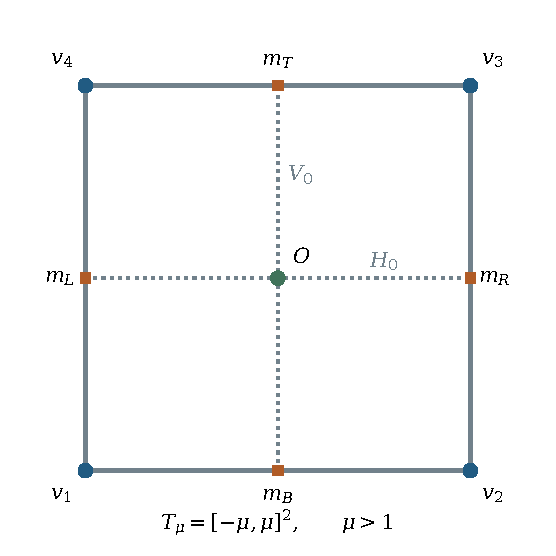
\includegraphics[width=.67\textwidth]{figures/01_target.pdf}
\caption{The fixed target and six-line grid. Corner indices determine the
geometric roles; discovery-round indices are only source locators.}
\label{fig:target}\end{figure}

